\documentclass[a4paper]{scrreprt}
\usepackage{scrextend}
\usepackage[german]{babel}
\usepackage[utf8]{inputenc}
\usepackage[T1]{fontenc}
\usepackage{ae}
\usepackage[bookmarks,bookmarksnumbered]{hyperref}

%graphics
\usepackage{graphicx}
\graphicspath{ 
  {images/high-level/}
   {images/CBMC/}
   {images/C-Editor/}
  } 
\usepackage[printonlyused]{acronym}
\usepackage{hyperref}
\usepackage{float}

\begin{document}

\title{Entwurf}
\author{Überdurchschnittliche Gruppe}
\maketitle 
\chapter{Übersicht}
\section{Einleitung}
Dieses Dokument beschreibt den Entwurf des Softwaresystemes welches in unserem Pflichtenheft beschrieben wurde. Es verwendet eine objektorientierte Architektur nach dem Model-View-Controller Prinzip. Zusammengehörige Funktionalität wird in Klassen gekapselt. Module sollen leicht austauschbar sein und klar definierte Schnittstellen bieten. Der Entwurf strebt an, modular und damit leicht veränder- und erweiterbar zu sein.

\subsection{abstrakteste Sichtweise} \label{abstract_section}
Die allgemeinste Sicht auf unser Softwaresystem ist Folgende: Wir benötigen
\begin{itemize}
\item Eine "'Quelle"' für eine Beschreibung eines Wahlverfahrens
\item Eine "'Quelle"' für eine Beschreibung der formalen Eigenschaften, welche diese Wahlverfahren erfüllen soll		
\item Eine Überprüfungsinstanz welche Wahlverfahren und Eigenschaften entgegennimmt das Ergebnis der Überprüfung zurückgibt
\item Eine Komponente welche diese Ergebnisse darstellen kann
\item Ein Koordinator, welcher die Koordination zwischen obigen Komponenten übernimmt
\end{itemize}

\begin{figure}[H]
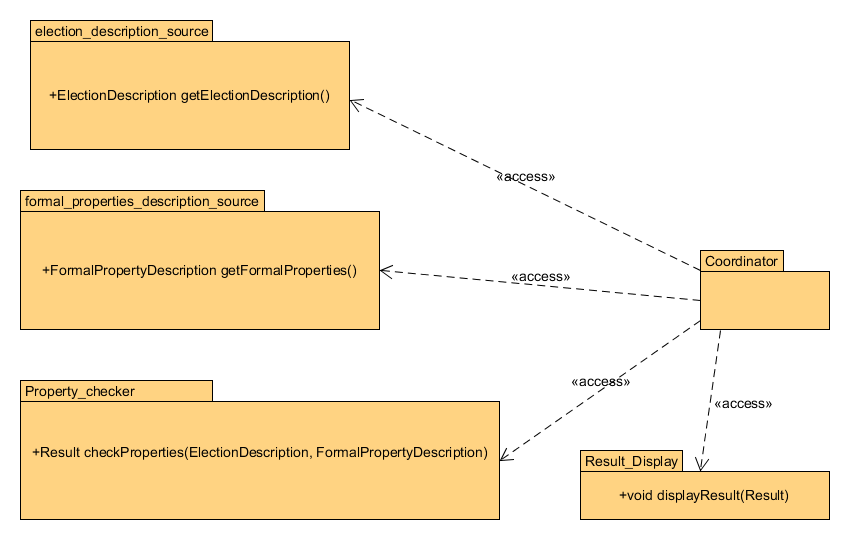
\includegraphics[scale=0.5]{highest-level-general-view.png}
\caption{allgemeinste Sicht auf die Architektur von BEAST}
\label{most_general_view_of_beast_architecture}
\end{figure}

\subsection{Konkrete Sichtweise} \label{concrete_section}
Der Vorteil der abstrakten Beschreibung ist, dass sie quasi unbegrenzte Möglichkeiten liefert und es sehr klar macht, an welchen Stellen man das Programm fundamental ändern kann. Wir werden die Beschreibung des Wahlverfahrens als C-Code implementieren, und die Quelle dafür als C-Editor. Es ist jedoch denkbar, dies in Zukunft durch einen graphischen Editor zu ersetzen, welcher zum Beispiel Flowcharts verwendet. Die formalen Eigenschaften wird in der im Pflichtenheft beschriebenen Syntax gegeben. Als Quelle dient die Eigenschaftenliste welche wiederum den Eigenschafteneditor verwendet. Die Koordination wird von dem Parametereditor übernommen. Zur Überprüfung wird ein bounded model checker verwendet, in unserem Fall speziell der C bounded model checker. Darstellen der Ergebnisse geschieht in der Eigenschaftenliste.  

\begin{figure}[H]
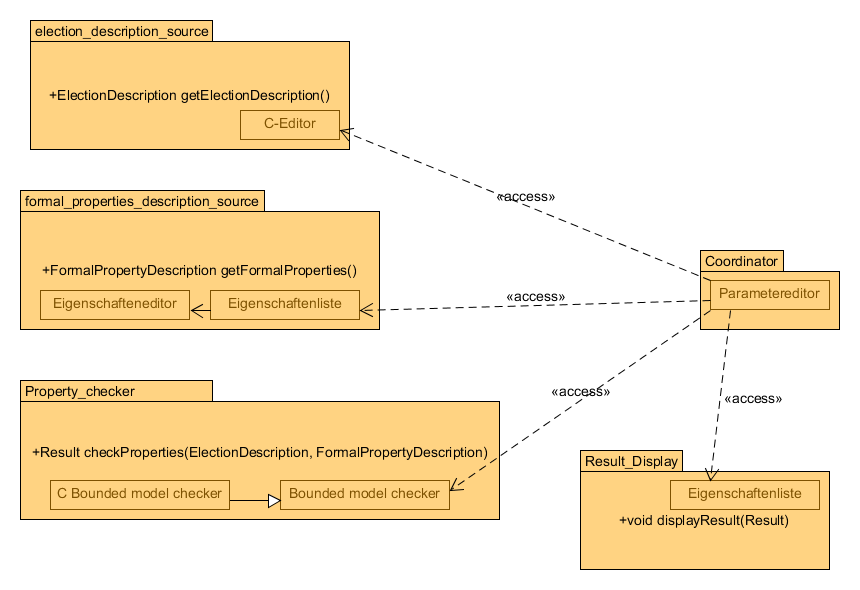
\includegraphics[scale=0.5]{highest-level-concrete-view.png}
\caption{Konkrete Sicht auf die Architektur von BEAST}
\label{concrete_view_of_beast_architecture}
\end{figure}

Genauer besitzen die Packete C-Editor, Eigenschaftenliste und CBMC-Schnittstelle jeweils Klassen, welche diese abstrakte Sichtweise widerspiegeln. Über diese wird die Kommunikation zwischen den Paketen ablaufen, gesteuert von dem Parametereditor.

\begin{figure}[H]
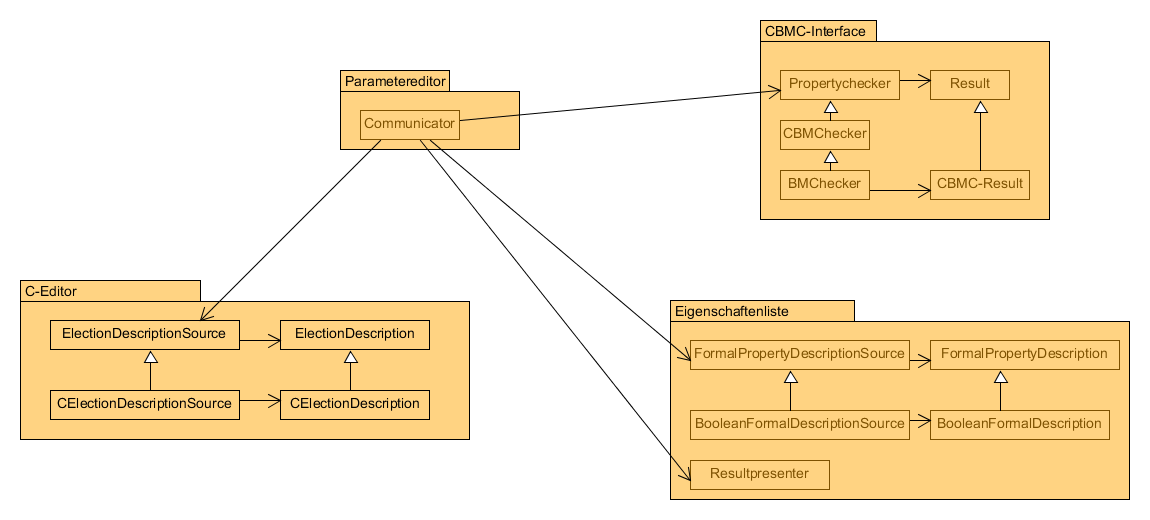
\includegraphics[scale=0.4]{high-level-communication.png}
\caption{Überblick über die Kommunikation zwischen den Paketen zum Überprüfen der Eigenschaften}
\label{view_of_communication_checking_formal_props}
\end{figure}

\begin{figure}[H]
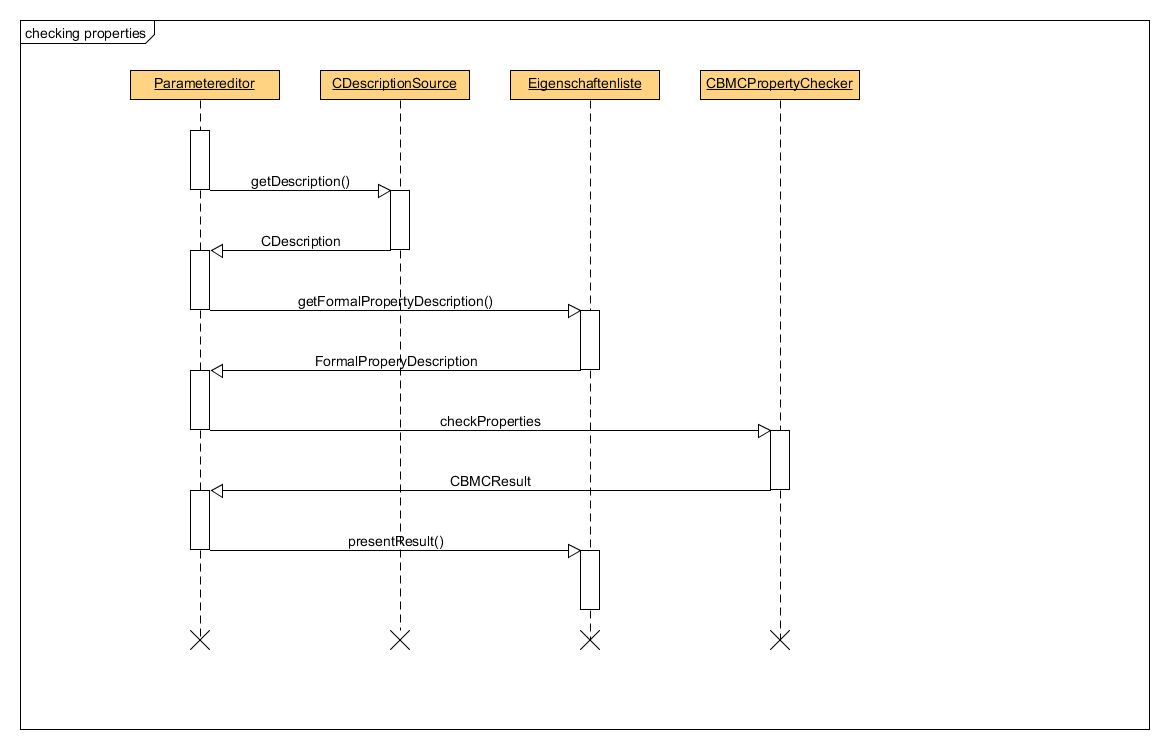
\includegraphics[scale=0.35]{high-level-communication-activity.png}
\caption{Zeitlicher Ablauf der Kommunikation}
\label{view_of_communication_checking_formal_props_activity_diagram}
\end{figure}

\subsection{Komplikationen im konkreten Fall}
Eine Trennung wie sie in \ref{abstract_section} und \ref{concrete_section} dargestellt wird ist in unserem konkreten Fall nicht zu hundert Prozent praktikabel. Dies liegt daran, dass die Komponenten ansonsten einige Funktionalität duplizieren würden. Alle Komponenten benötigen Funktionalität zum Laden und Speichern von Dateien. C-Editor und Eigenschafteneditor haben beide Textpanels welche Code darstellen. Dieser muss in beiden Fällen auf bestimmte Art und Weiße formatiert werden und auf Fehler untersucht werden. Gefundene Fehler müssen in beiden Fällen im Code markiert werden. All diese mehrmals aufkommende Funktionalität wird in eigene Klassen gekapselt werden.

\section{Überblick über einzelne Komponenten}
Hier wird ein Überblick über die einzelnen Komponenten gegeben. Wie bereits erwähnt werden alle Komponenten nach dem Model-View-Controller Prinzip in Funktionalität untergliedert. Dies bewirkt eine Trennung der internen und für den Benutzer sichtbaren Darstellung der verschiedenen Daten. Darauf wird im Folgenden der Schwerpunkt gelegt. Darauf, wie die Funktionalität zwischen den Komponenten geteilt wird, wird noch nicht eingegangen.

\subsection{C-Editor}
Der C-Editor hat als hauptsächliche Komplikation die Tatsache, dass sowohl die Darstellung des Code (View) als auch die Eingabe des Benutzers (Controller) als auch interne Darstellung des Codes als String (Model) zunächst durch eine Komponente - die JTextPane - übernommen werden. Dies hat den Vorteil, dass viel Funktionalität bereitgestellt wird: Kopieren, Löschen, Ausschneiden von Text. Der Nachteil ist wenig Flexibilität den Text während der Eingabe zu bearbeiten. Daher werden diese Funktionen getrennt bearbeitet werden. Die Keypress - Events werden nicht mehr direkt an die Textpane weitergeleitet sondern zunächst abgefangen. Der Code wird intern in einem speziellen Format abgespeichert. Dieses feuert ein Event wann immer der Code aktualisiert wird oder Fehler im Code festgestellt werden. Dieses Event wird von dem TextPaneDecorator abgefangen, der den Code dann darstellt und sich um das Syntax Highlighting kümmert. 
\subsubsection{Controller}
Der Controller ist Vermittlungsschicht zwischen View und Model. Um dies zu erledigen

\begin{figure}[H]
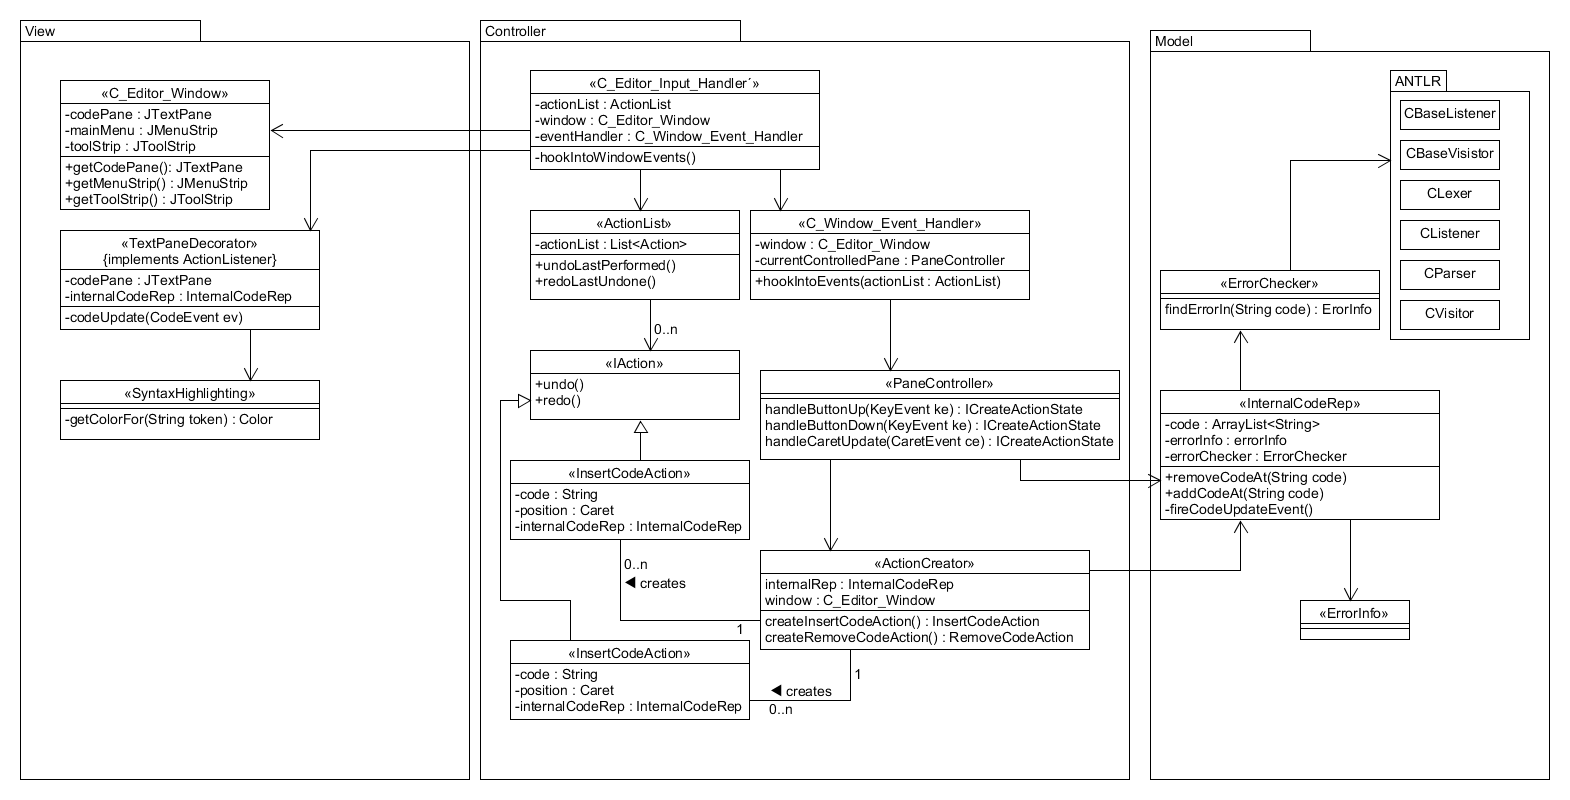
\includegraphics[scale=0.4, angle = 270]{CEditorMVC.png}
\caption{C-Editor overview}
\label{C-Editor-MVC-overview}
\end{figure}

\chapter{Überprüfung der Modelle}
Blabla bounded model blabla cbmc

\begin{figure}[H]
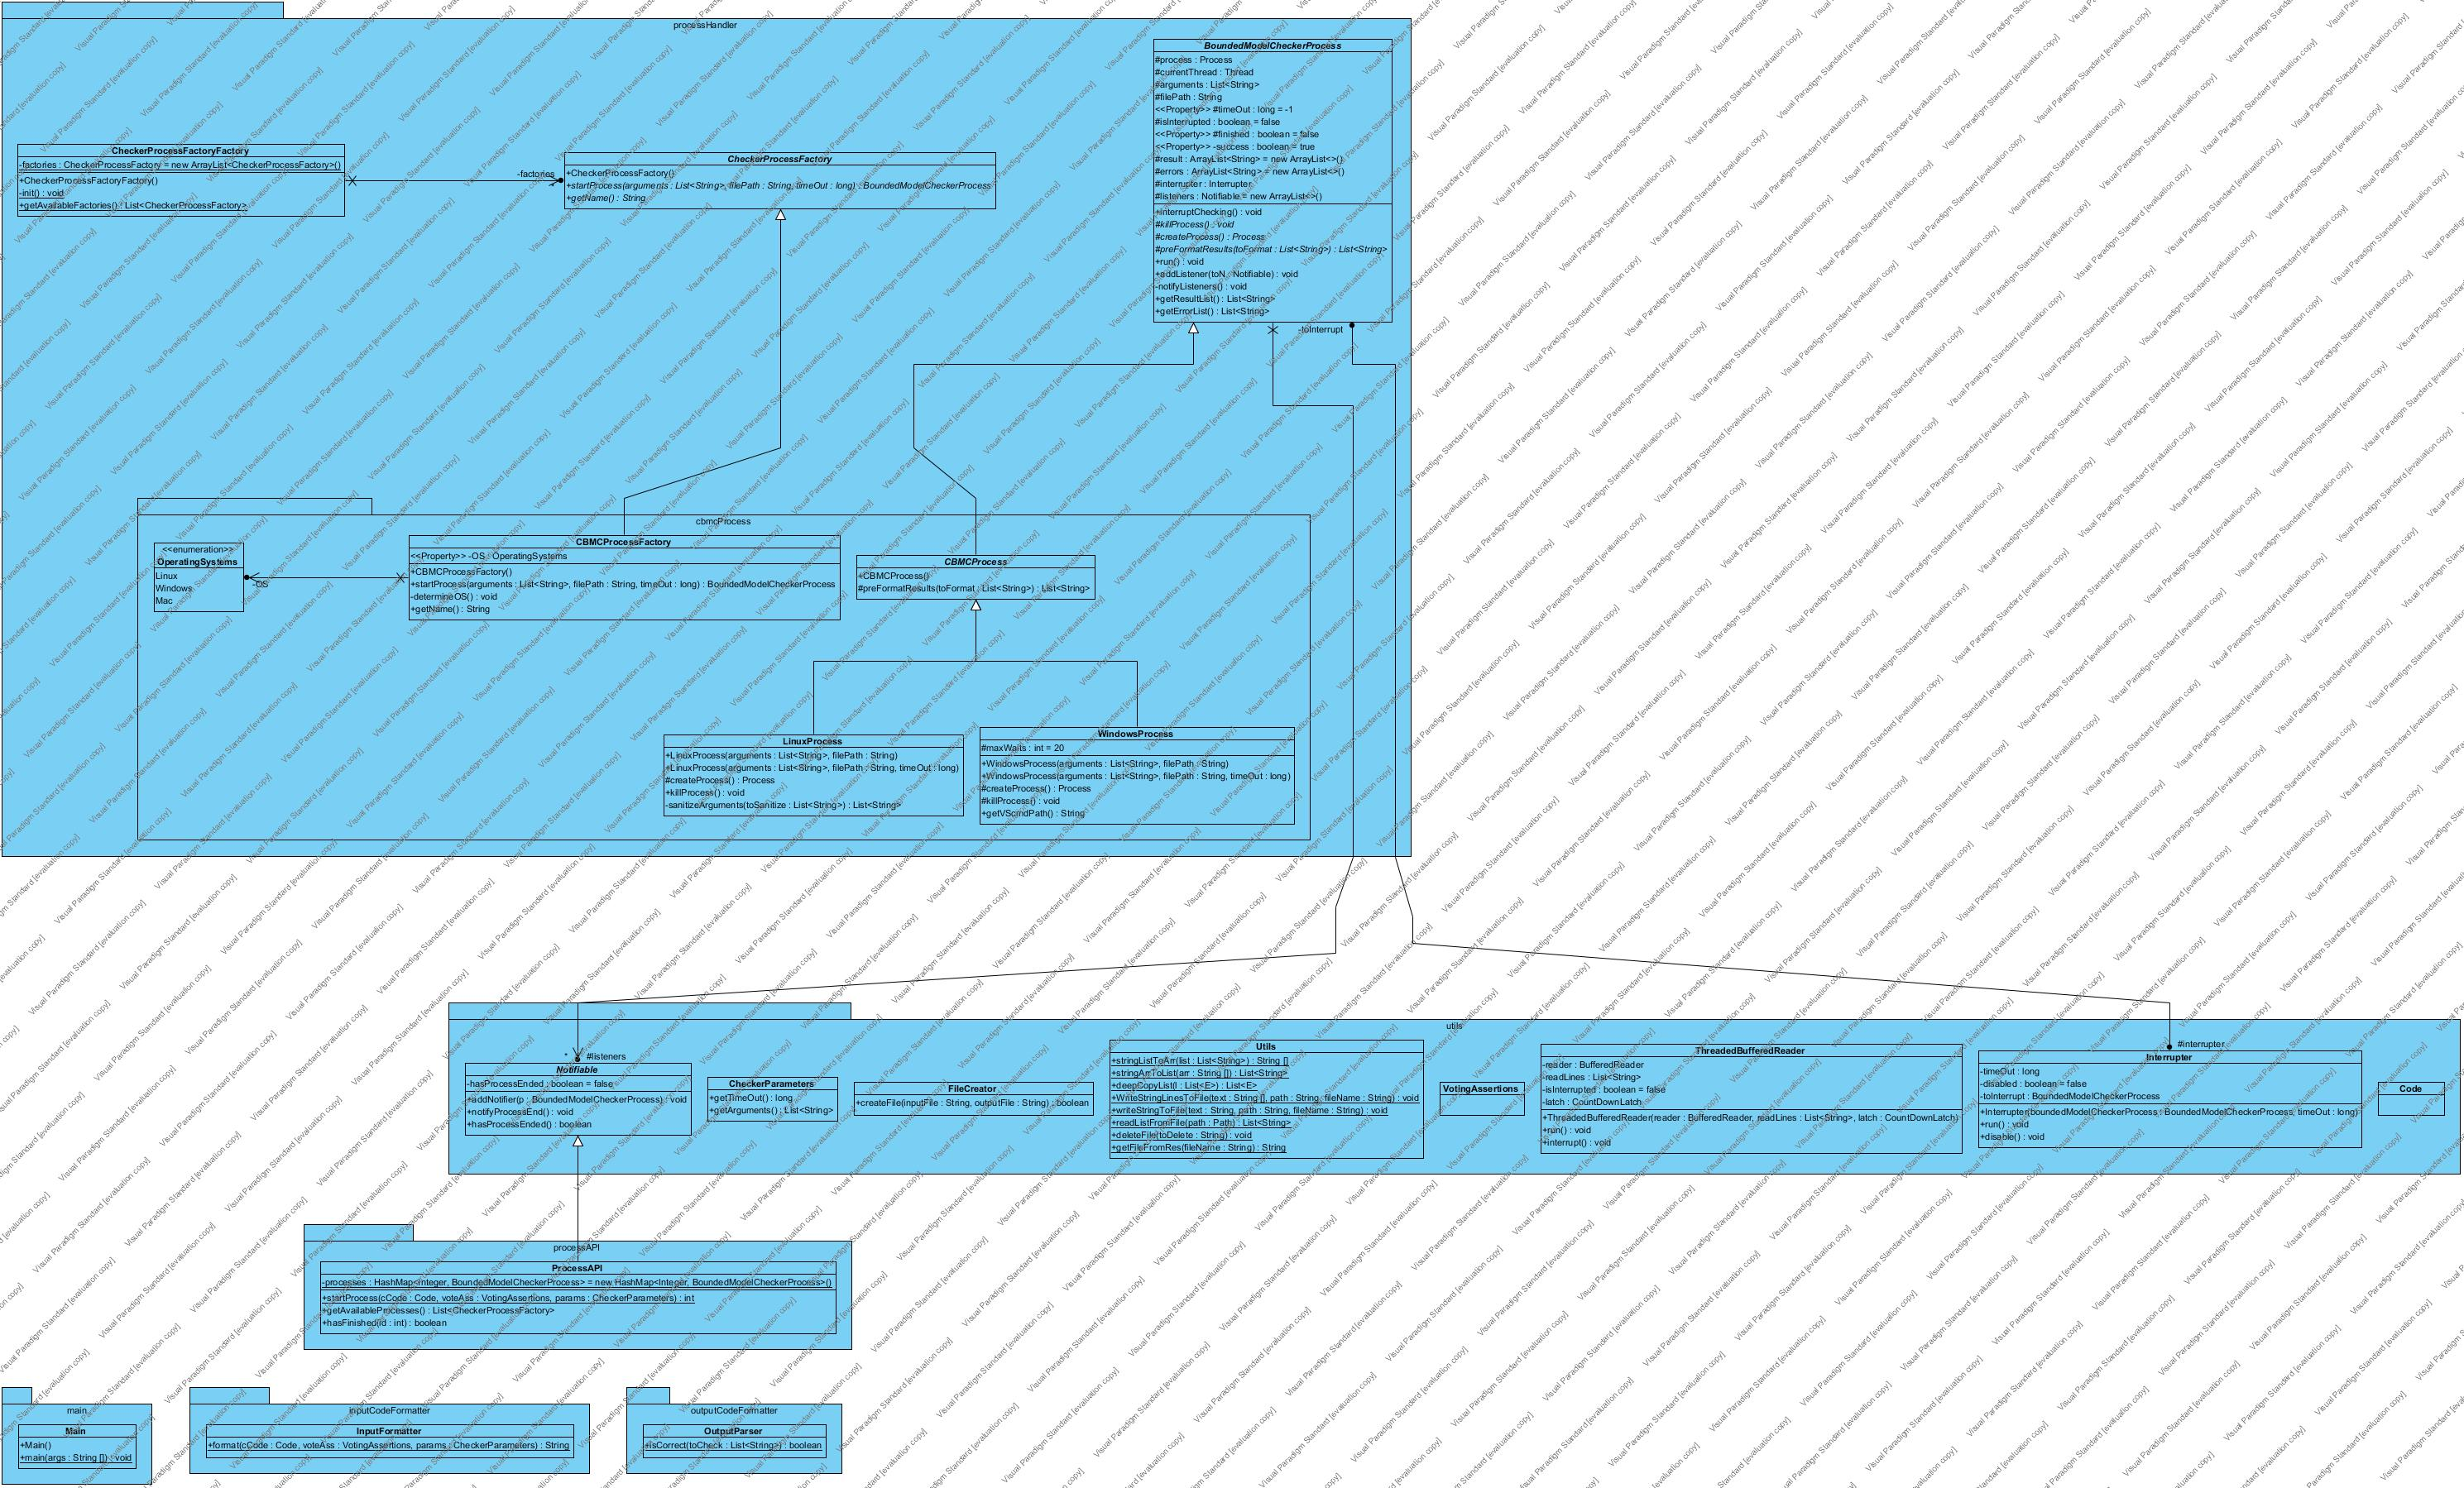
\includegraphics[scale=0.25, angle = 270]{cbmcDiagram.jpg}
\caption{CBMC Schnittstelle}
\label{concrete_view_of_beast_architecture}
\end{figure}




\end{document}
